%%%%%%%%%%%%%%%%%%%%%%%%%%%%%%%%%%%%%%%%%
%% Section to host Figures
\section{Figures}
\label{sec:figures}

\begin{figure}[H]
    \centering
    \singlespacing
    \caption{Mean Total Funding among Public Universities, by Year.}
    \begin{subfigure}[b]{0.495\textwidth}
        \centering
        \caption{Total, \$ 2021 CPI-U.}
        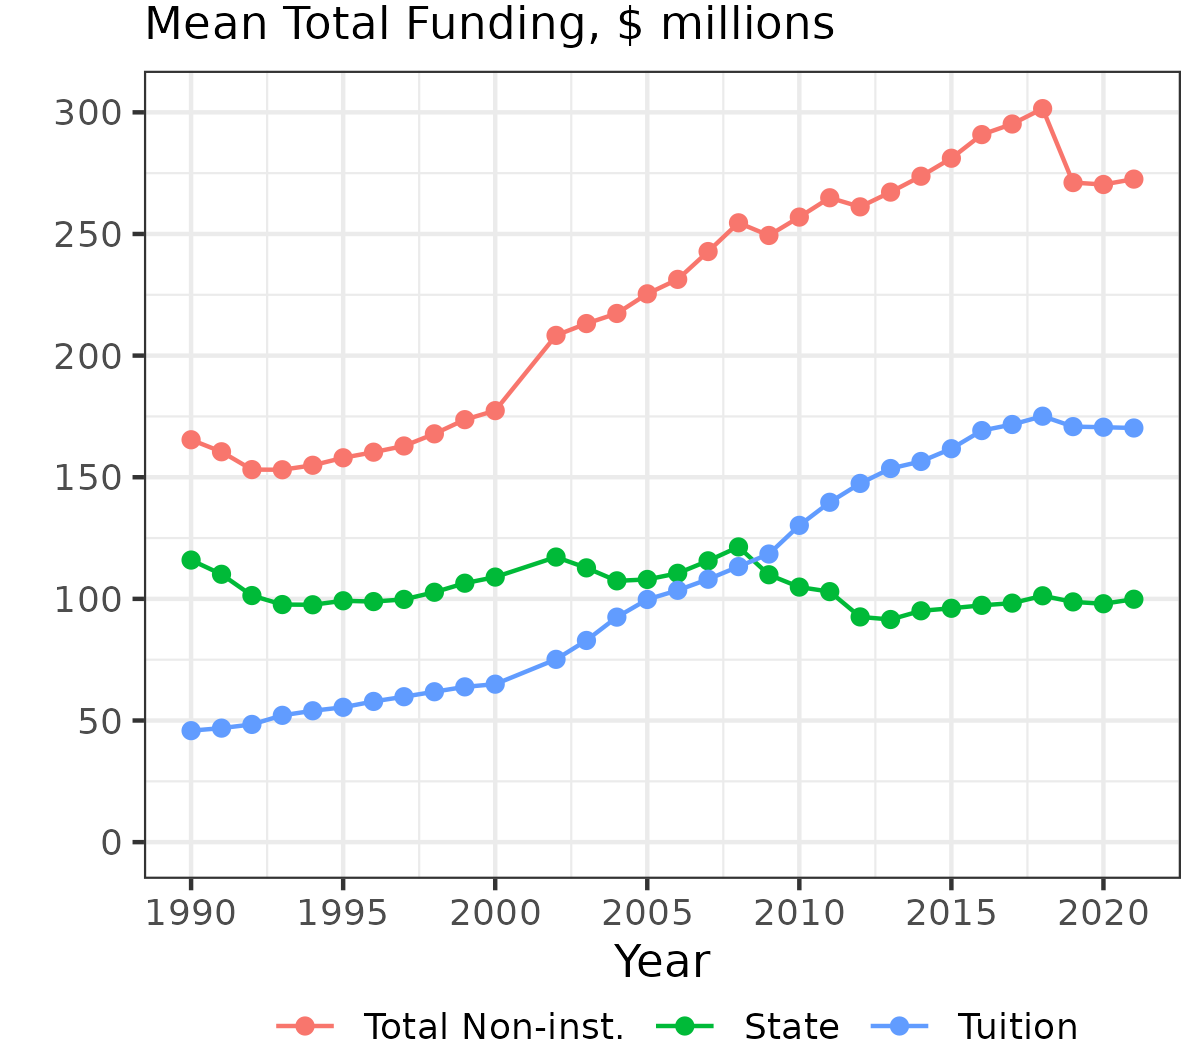
\includegraphics[width=\textwidth]{figures/mean-funding-total.png}
        \label{fig:mean-funding-total}
    \end{subfigure}
    \begin{subfigure}[b]{0.495\textwidth}
        \centering
        \caption{Per Student, \$ 2021 CPI-U.}
        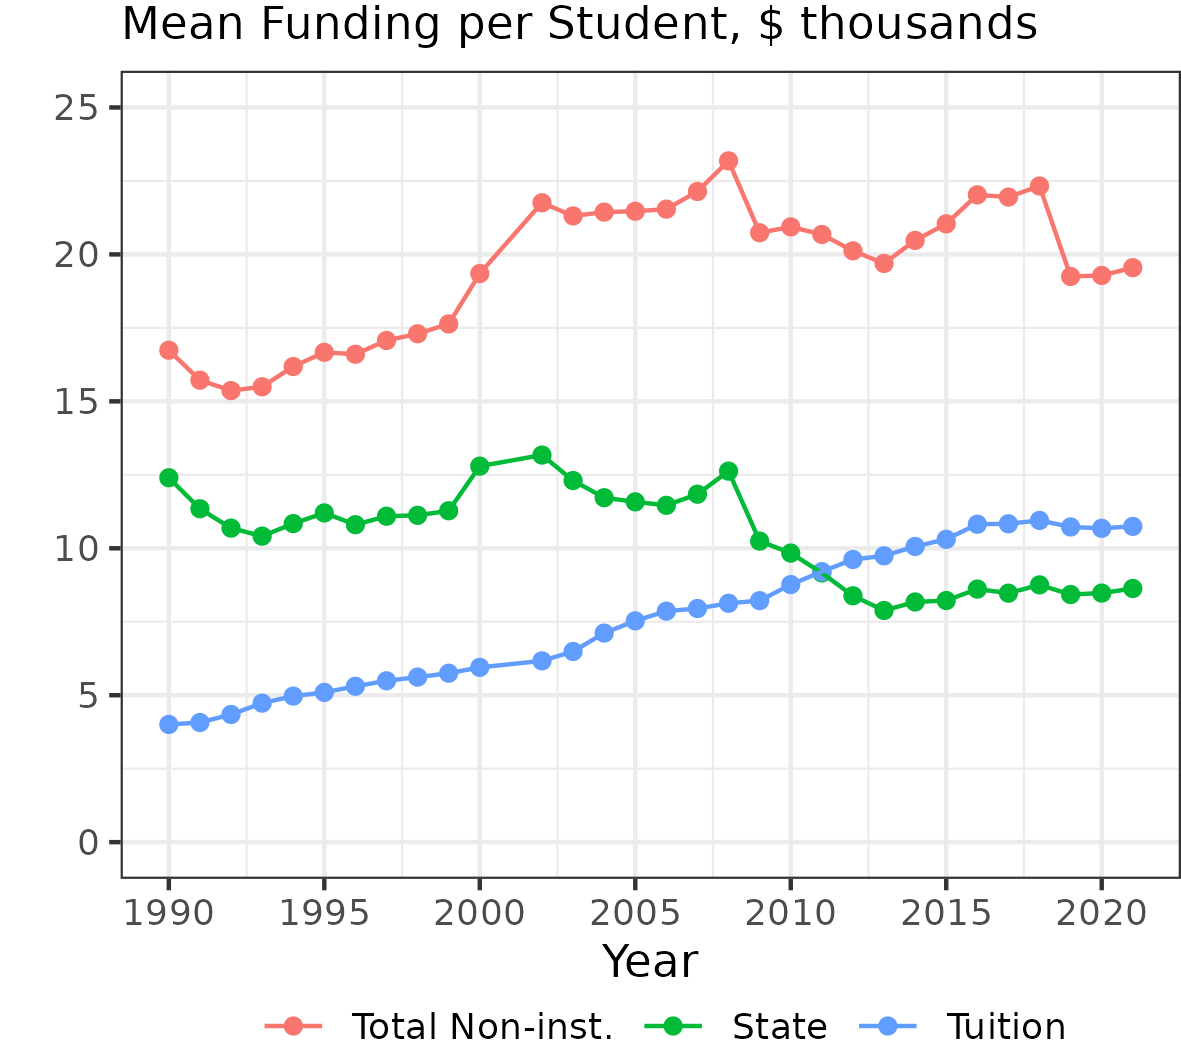
\includegraphics[width=\textwidth]{figures/mean-funding-fte.png}
        \label{fig:mean-funding-fte}
    \end{subfigure}
    \label{fig:funding}
    \justify
    \footnotesize
    \textbf{Note}:
    This figure shows the mean funding for US public universities as a total (in figure a.) and divided by student enrolment (figure b.).
    The numbers are adjusted to 2021 figures by CPI-U.
    Non-institutional revenues refers to the sum of federal, state, and local funding plus tuition revenues; these sum to the majority of university funding, but exclude numbers such as university income from capital projects.
    These figures are calculated with IPEDS data.
\end{figure}

\begin{figure}[H]
    \centering
    \singlespacing
    \caption{Total Student enrolment, by University Sector and Year.}
    \begin{subfigure}[b]{0.495\textwidth}
        \centering
        \caption{Total Enrolment, Nation-wide.}
        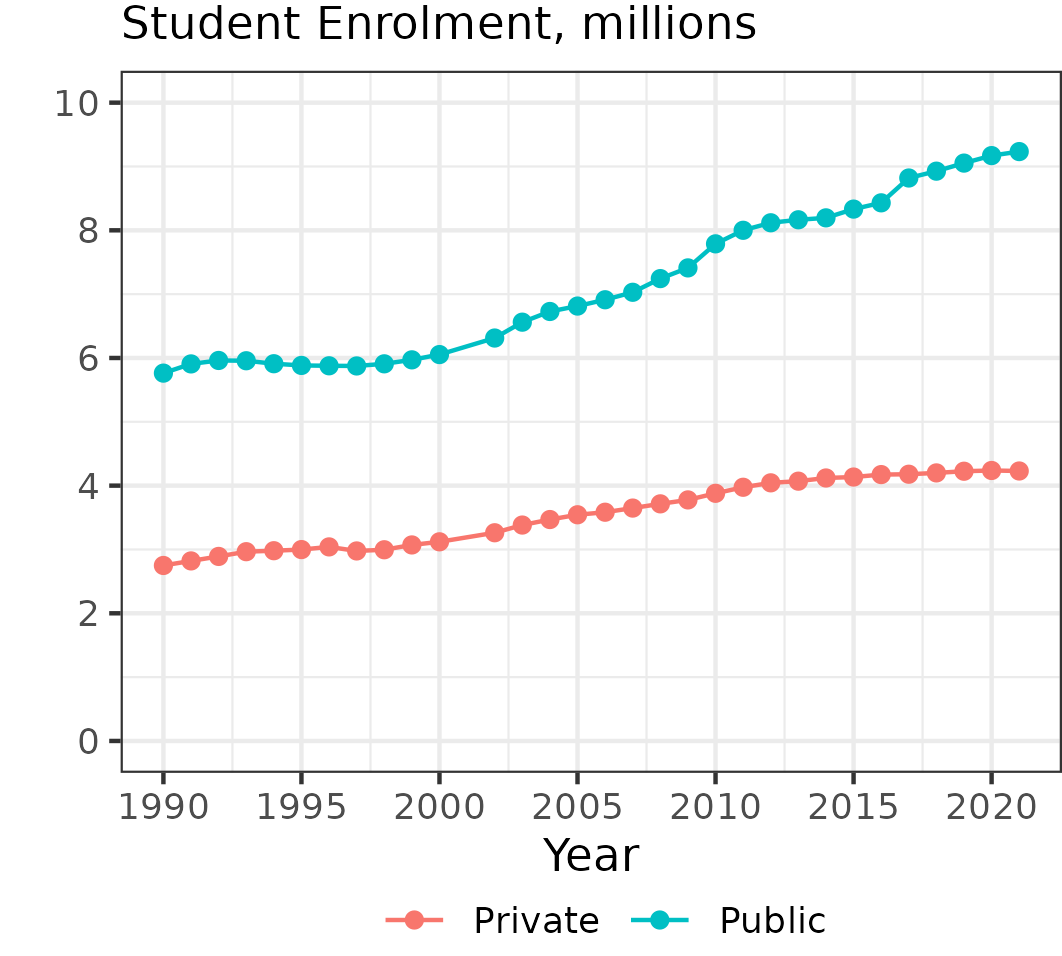
\includegraphics[width=\textwidth]{figures/enrollment-total.png}
        \label{fig:enrollment-total}
    \end{subfigure}
    \begin{subfigure}[b]{0.495\textwidth}
        \centering
        \caption{Mean Enrolment, per University.}
        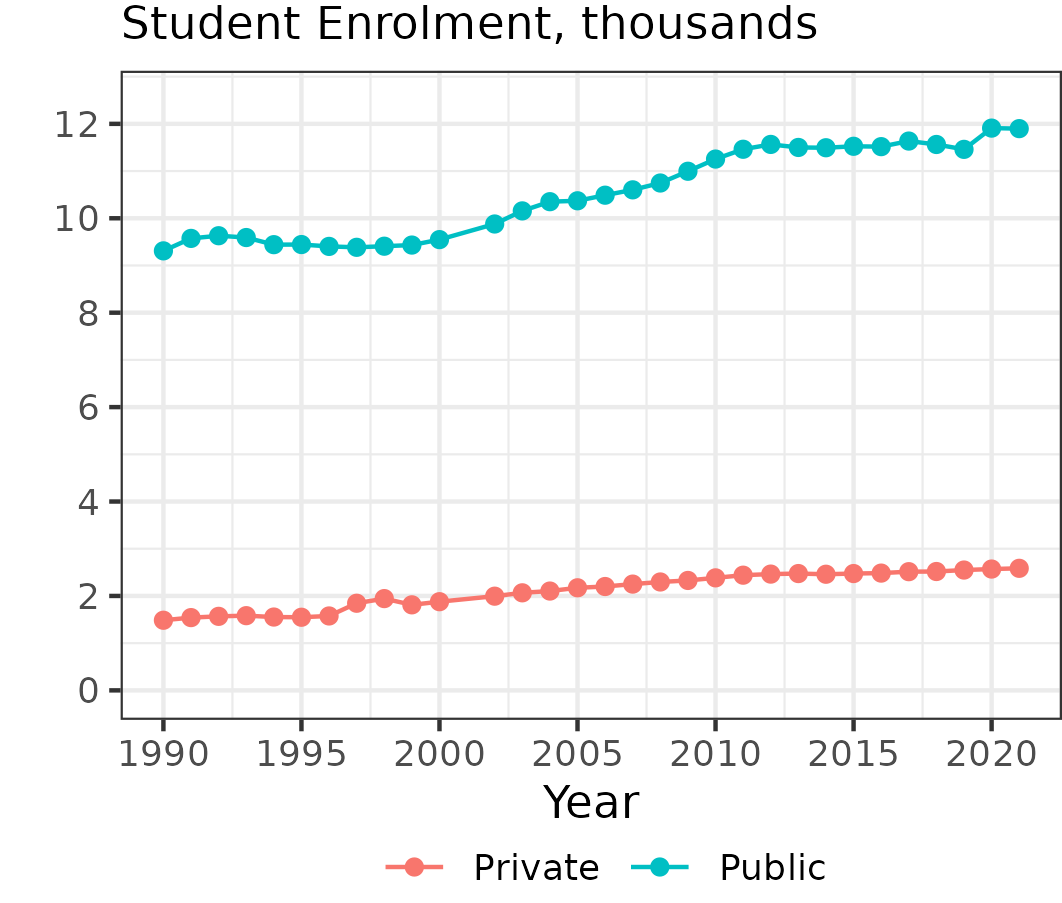
\includegraphics[width=\textwidth]{figures/enrollment-mean.png}
        \label{fig:enrollment-mean}
    \end{subfigure}
    \label{fig:enrolment}
    \justify
    \footnotesize
    \textbf{Note}:
    This figure shows the total and mean enrolment for US universities, comparing public and private universities.
    Most of the higher education enrolment increase for the last 30 years was in public universities, who continue to enrol the vast majority of higher education students in the US.
    These figures are calculated with IPEDS data.
\end{figure}

\newpage
\begin{figure}[H]
    \centering
    \singlespacing
    \caption{Trends in Mean Student Enrolment per Professor, by University Sector and Faculty level.}
    \begin{subfigure}[b]{0.495\textwidth}
        \centering
        \caption{Lecturer.}
        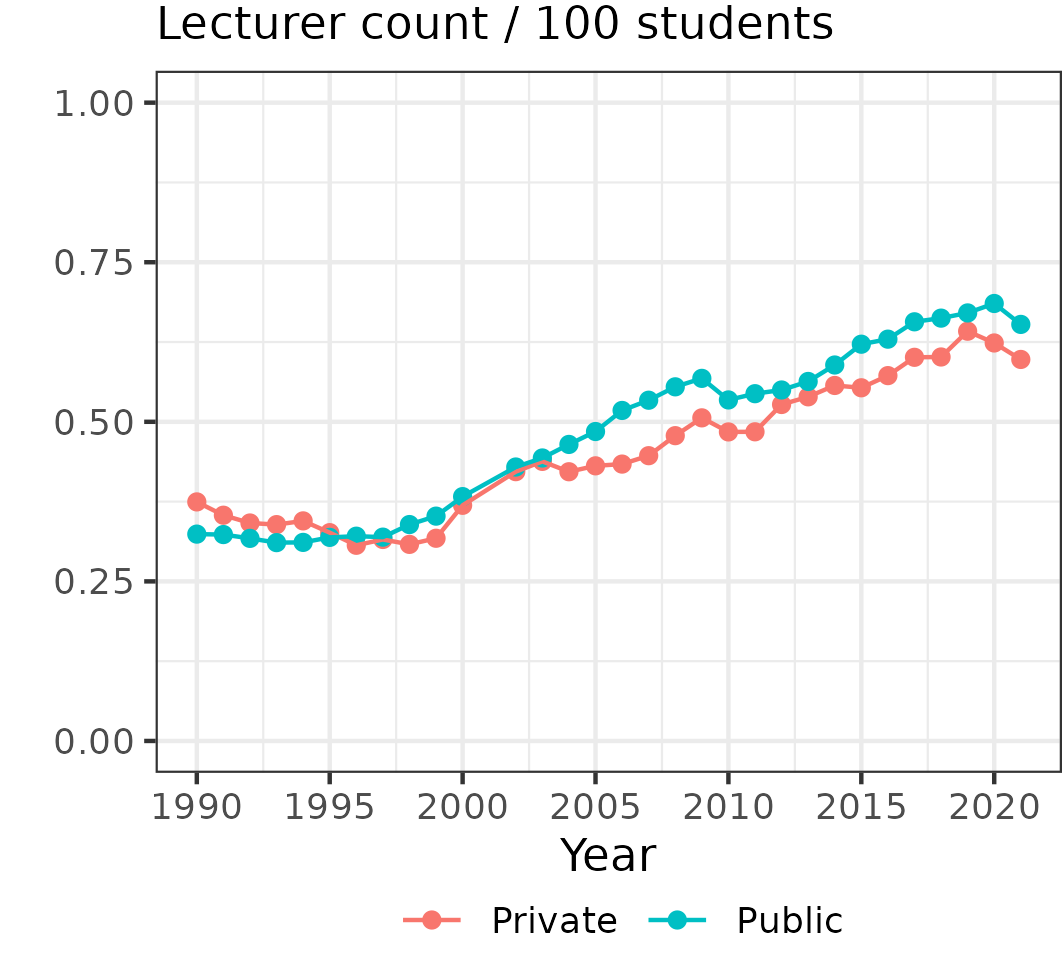
\includegraphics[width=\textwidth]{figures/lecturer-fte-perprof.png}
        \label{fig:lecturer-fte-perprof}
    \end{subfigure}
    \begin{subfigure}[b]{0.495\textwidth}
        \centering
        \caption{Assistant.}
        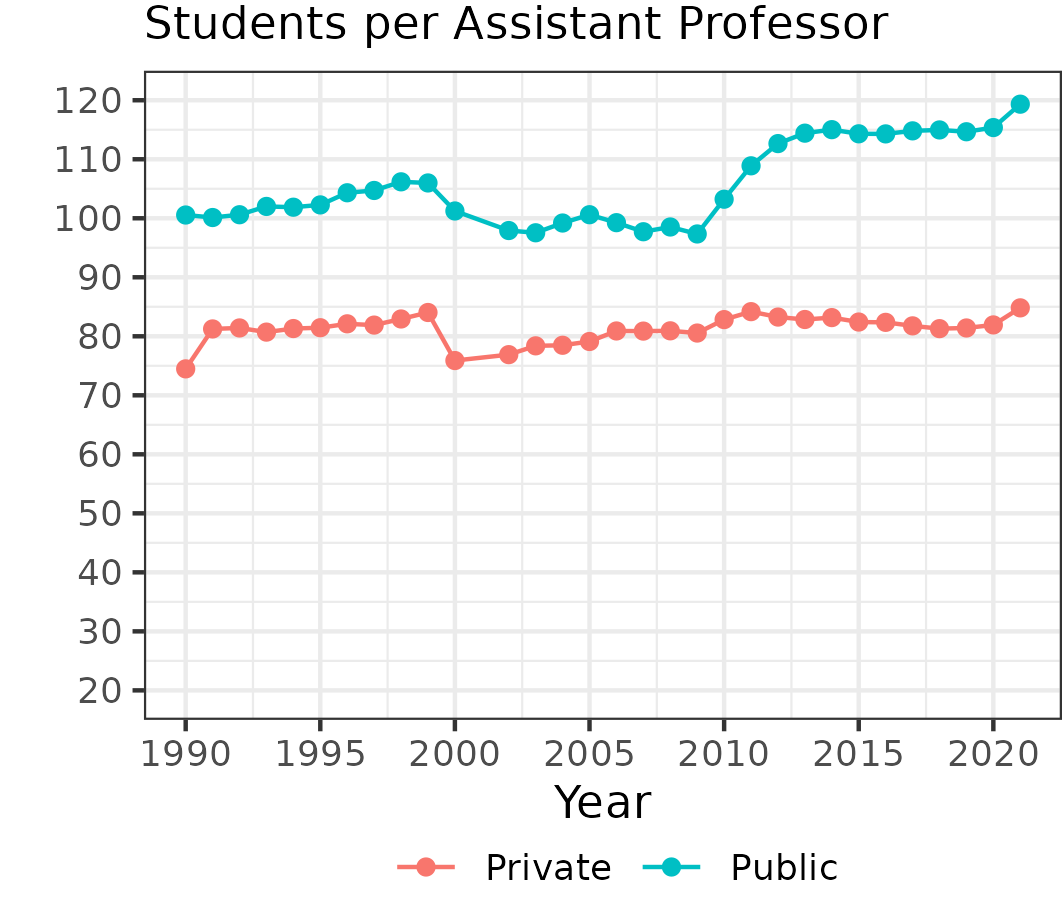
\includegraphics[width=\textwidth]{figures/assistant-fte-perprof.png}
        \label{fig:assistant-fte-perprof}
    \end{subfigure}
    \begin{subfigure}[b]{0.495\textwidth}
        \centering
        \caption{Full.}
        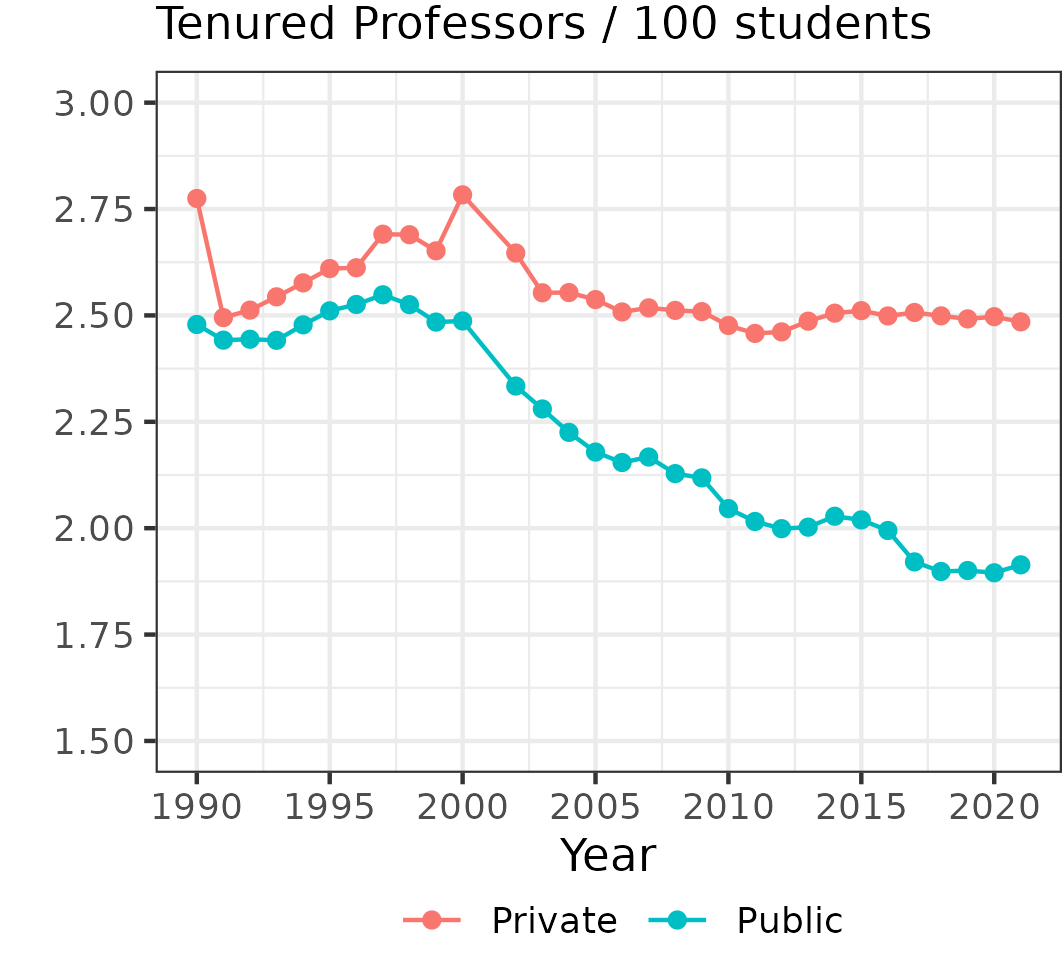
\includegraphics[width=\textwidth]{figures/full-fte-perprof.png}
        \label{fig:full-fte-perprof}
    \end{subfigure}
    \begin{subfigure}[b]{0.495\textwidth}
        \centering
        \caption{All.}
        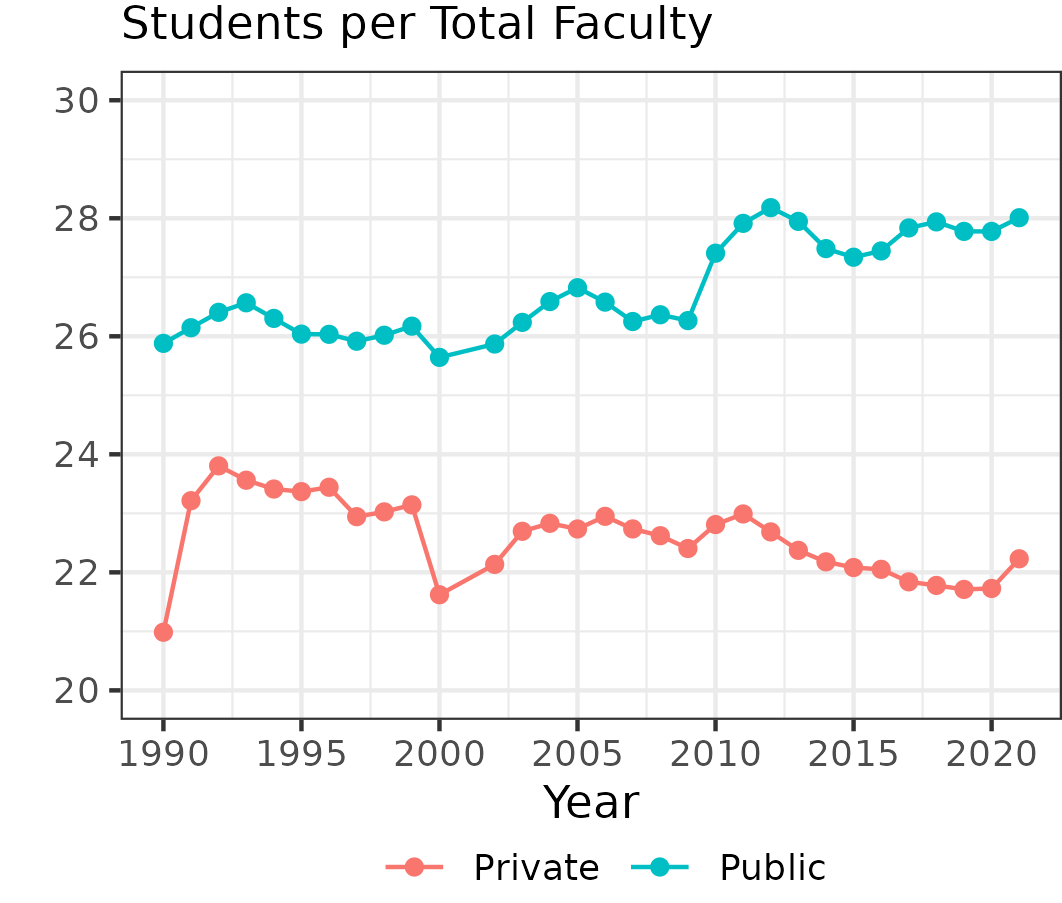
\includegraphics[width=\textwidth]{figures/all-fte-perprof.png}
        \label{fig:all-fte-perprof}
    \end{subfigure}
    \label{fig:fte-perprof}

    \justify
    \footnotesize
    \textbf{Note}:
    This figure shows the average number of students per faculty member, by different faculty position, at US public universities.
    E.g., panel A calculates the mean of (lecturer count) / (student enrolment) at US public universities, for each year of 1990--2017, to show the average trend in faculty composition compared to student enrolment.
    These figures are calculated with IPEDS data.
\end{figure}

\newpage
\begin{figure}[H]
    \centering
    \singlespacing
    \caption{Mean Funding Sources among Illinois Public Universities, by Year.}
    \begin{subfigure}[b]{0.495\textwidth}
        \centering
        \caption{Total, \$ 2021 CPI-U.}
        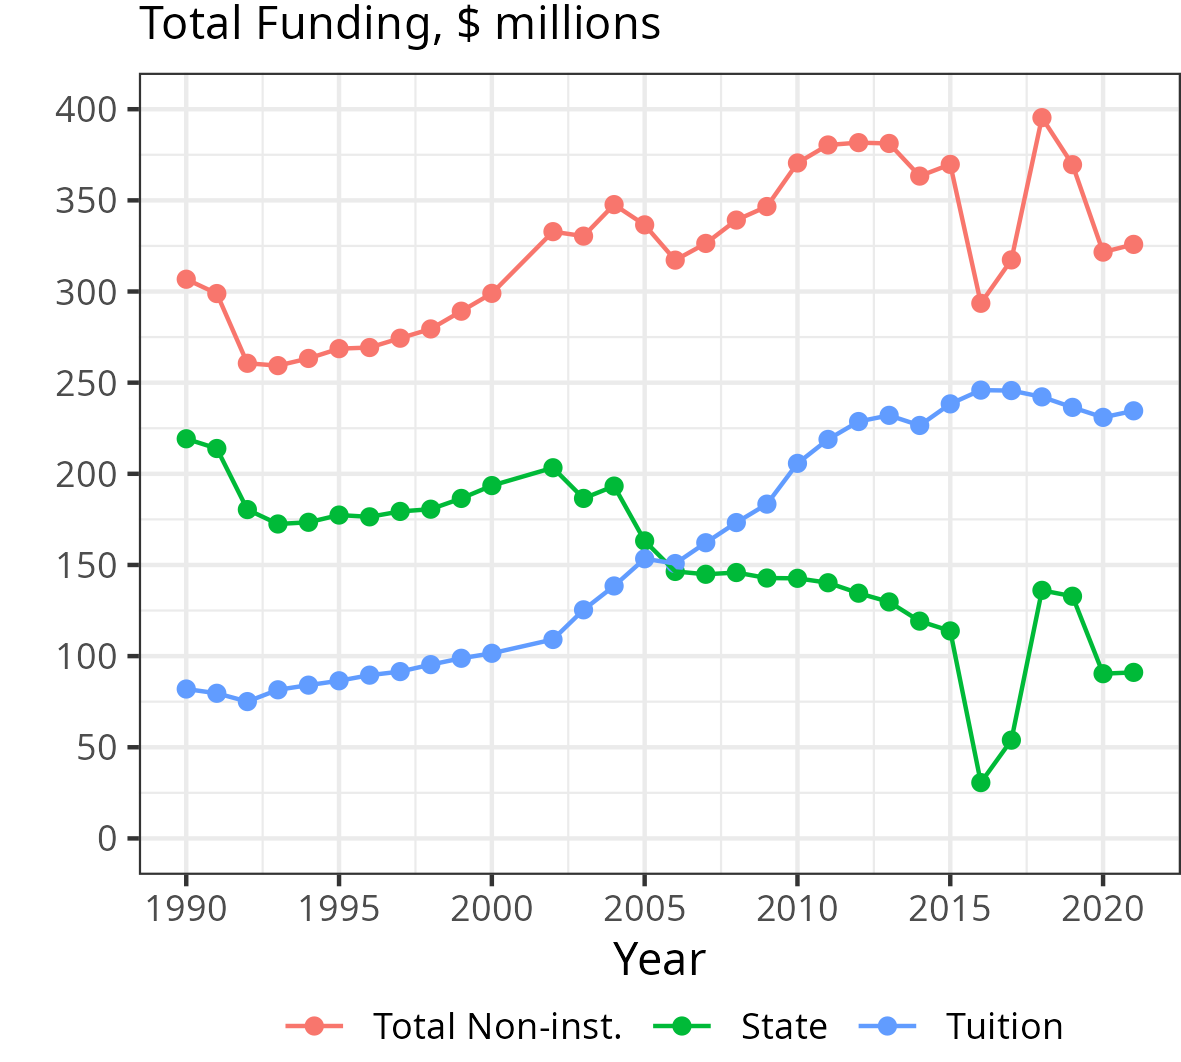
\includegraphics[width=\textwidth]{figures/illinois-funding-total.png}
        \label{fig:illinois-funding-total}
    \end{subfigure}
    \begin{subfigure}[b]{0.495\textwidth}
        \centering
        \caption{Per Student, \$ 2021 CPI-U.}
        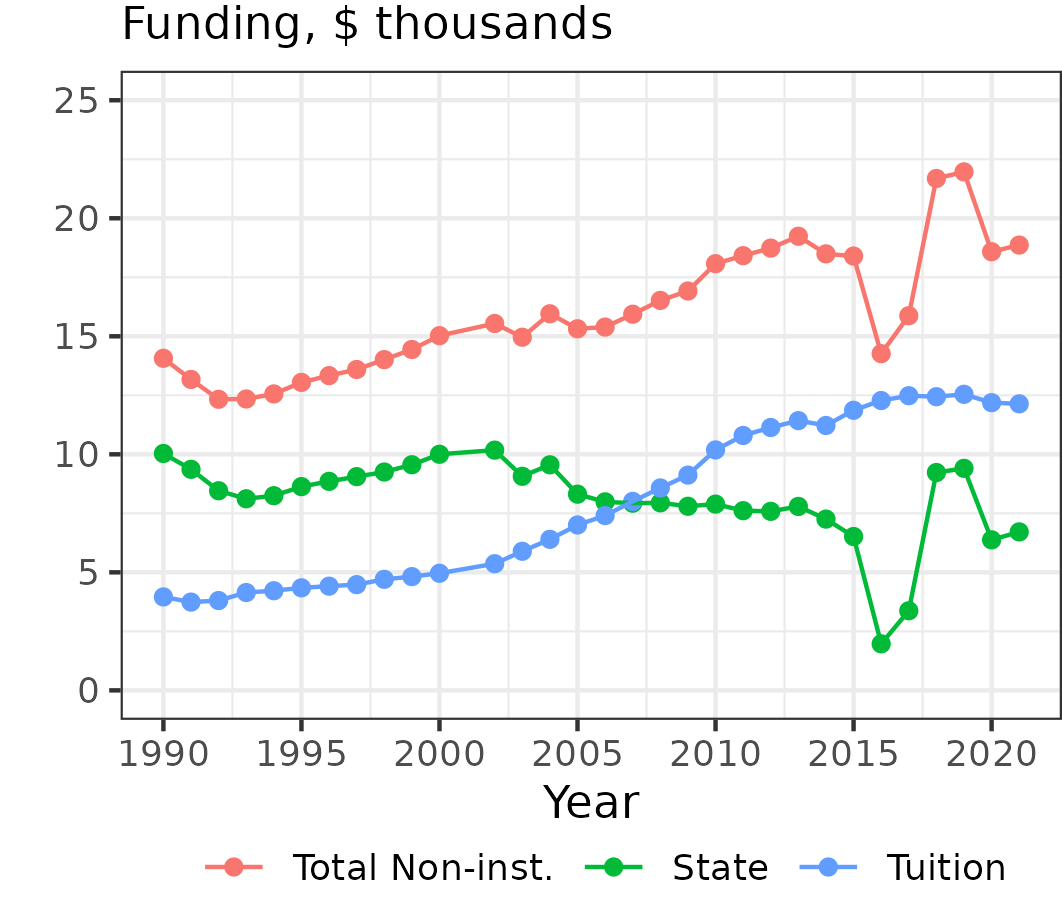
\includegraphics[width=\textwidth]{figures/illinois-funding-fte.png}
        \label{fig:illinois-funding-fte}
    \end{subfigure}
    \label{fig:illinois-funding}

    \justify
    \footnotesize
    \textbf{Note}:       
    This figure shows the mean funding for Illinois public universities as a total (in figure a.) and divided by student enrolment (figure b.).
    The numbers are adjusted to 2021 figures by CPI-U.
    Non-institutional revenues refers to the sum of federal, state, and local funding plus tuition revenues; these sum to the majority of university funding, but exclude numbers such as university income from capital projects.
    These figures are calculated with IPEDS data.
\end{figure}

\newpage
\begin{figure}[H]
    \centering
    \singlespacing
    \caption{Local Projection Estimates for Effect of State Funding on Faculty Count per Student at Universities, by Professor Group.}
    \begin{subfigure}[b]{0.495\textwidth}
        \centering
        \caption{Lecturers.}
        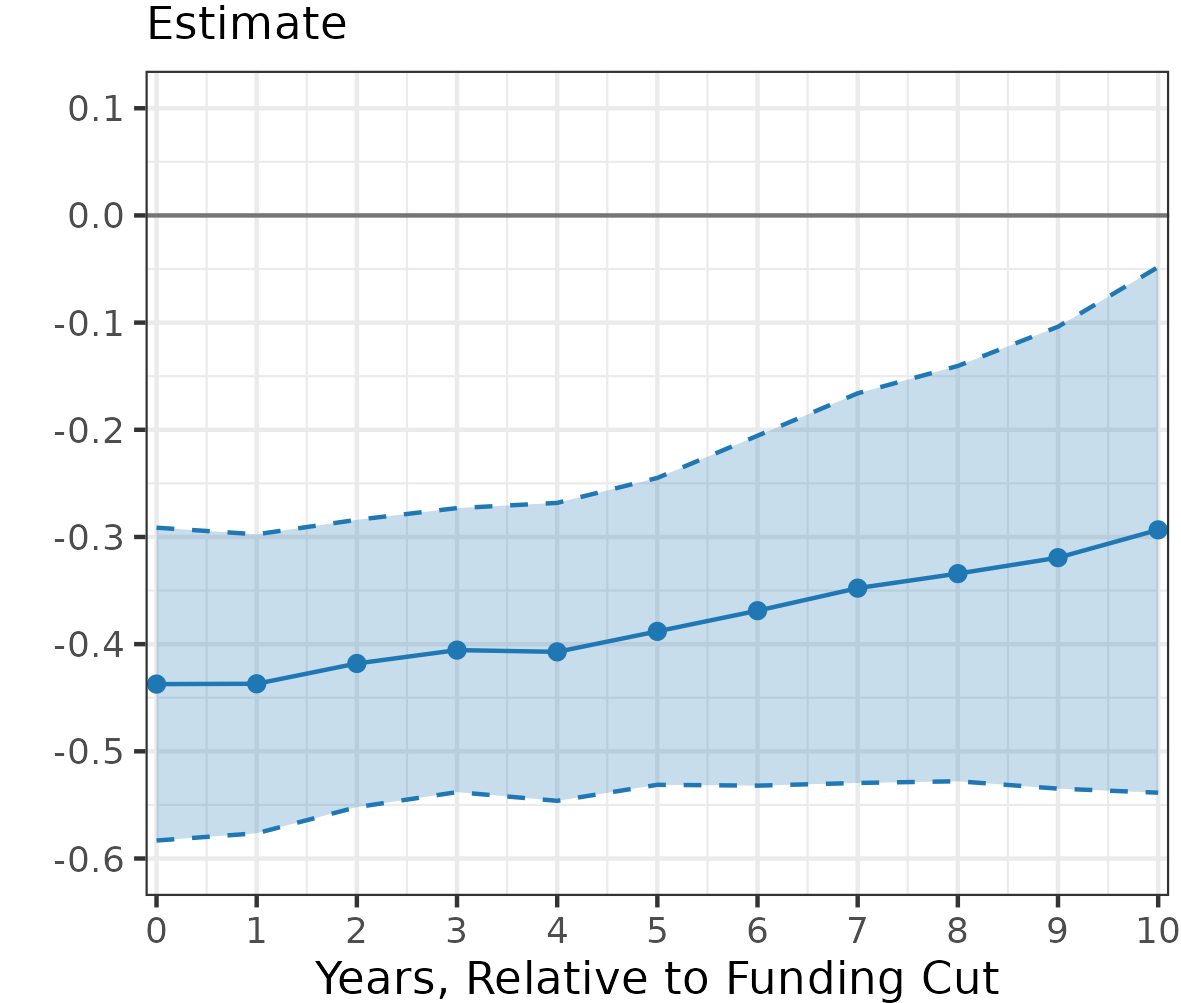
\includegraphics[width=\textwidth]{figures/lecturer-count-lp.png}
        \label{fig:lecturer-count-lp}
    \end{subfigure}
    \begin{subfigure}[b]{0.495\textwidth}
        \centering
        \caption{Assistant Professors.}
        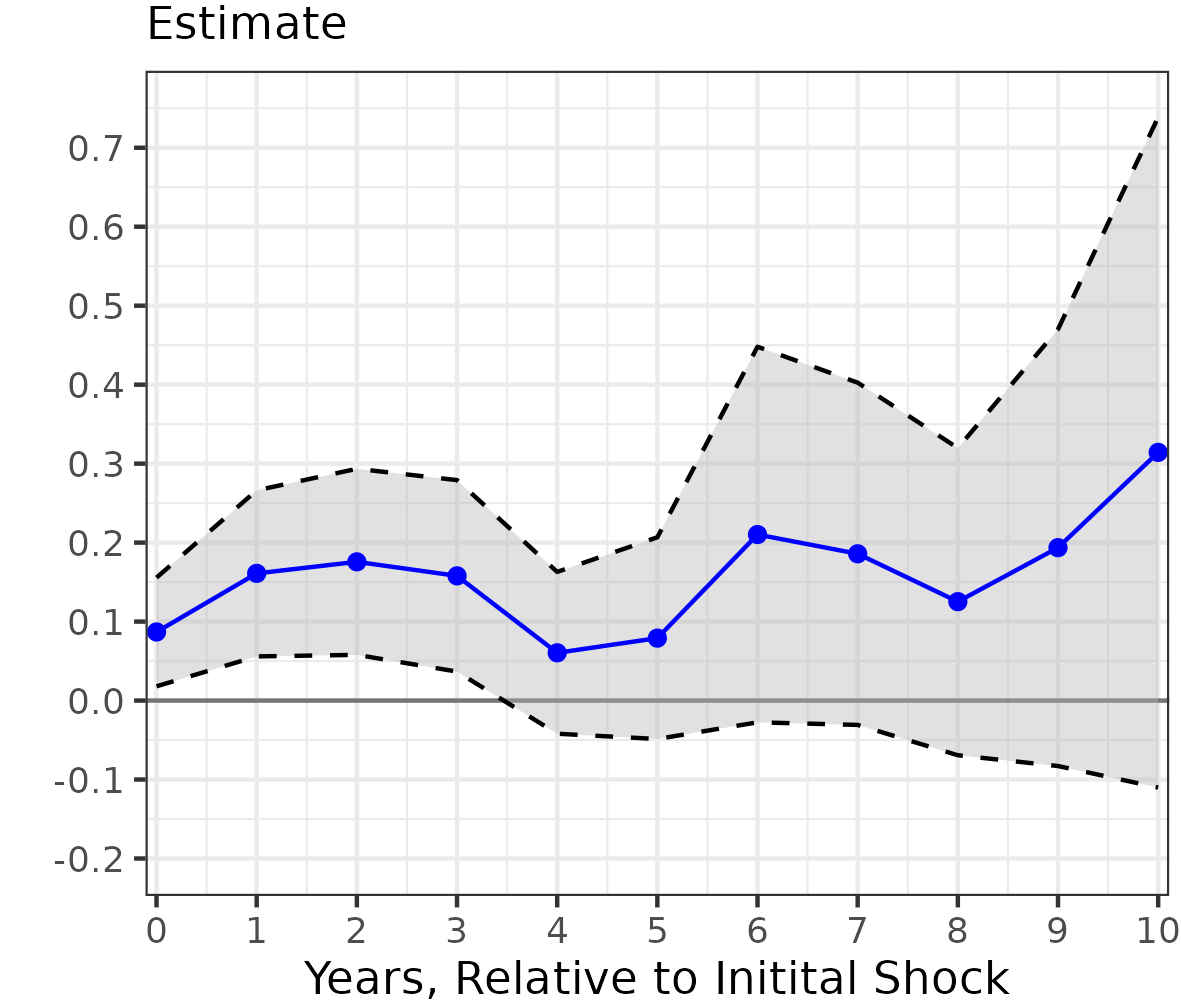
\includegraphics[width=\textwidth]{figures/assistant-count-lp.png}
        \label{fig:assistant-count-lp}
    \end{subfigure}
    \begin{subfigure}[b]{0.495\textwidth}
        \centering
        \caption{Full Professors.}
        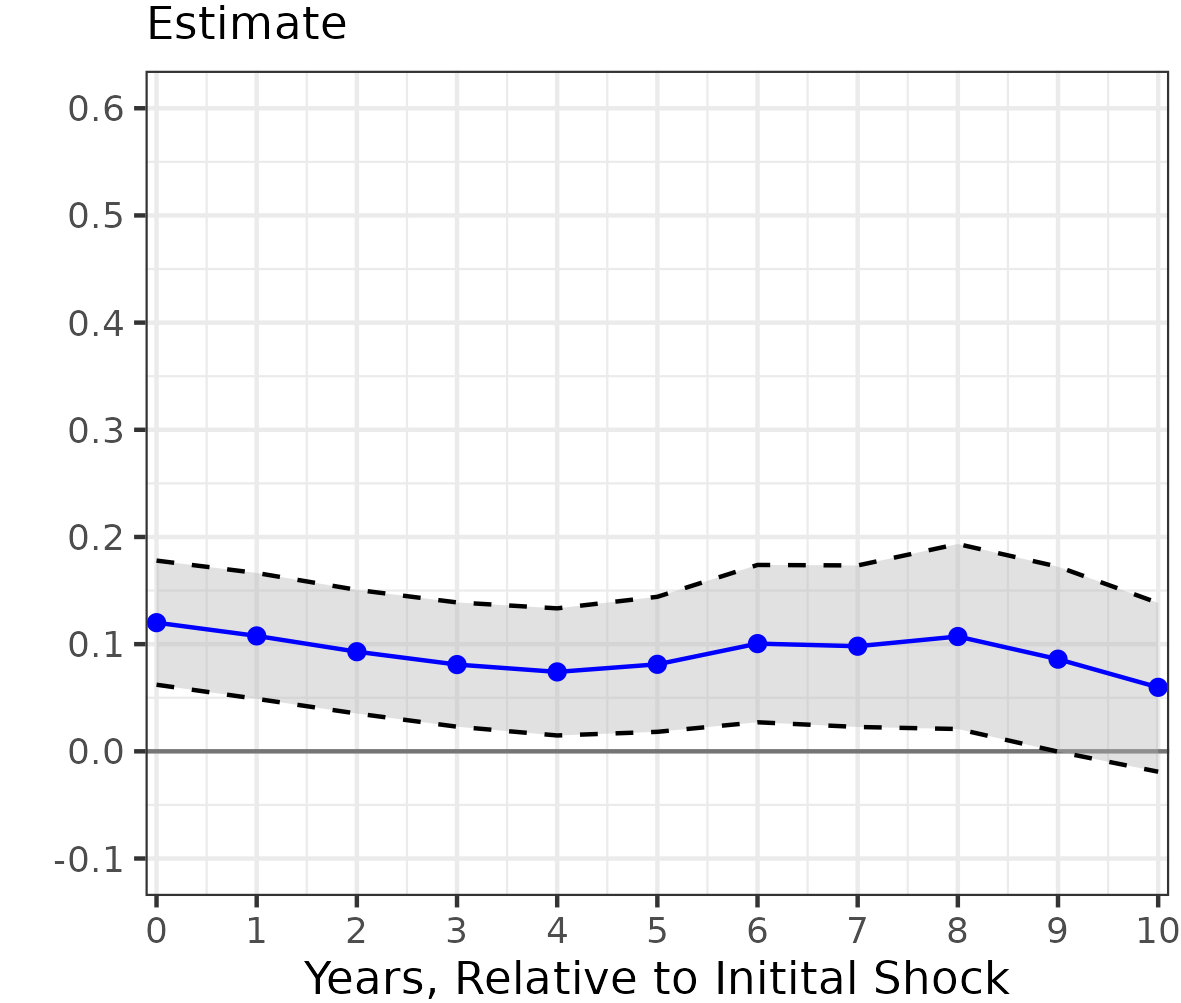
\includegraphics[width=\textwidth]{figures/full-count-lp.png}
        \label{fig:full-count-lp}
    \end{subfigure}
    \begin{subfigure}[b]{0.495\textwidth}
        \centering
        \caption{All Professors.}
        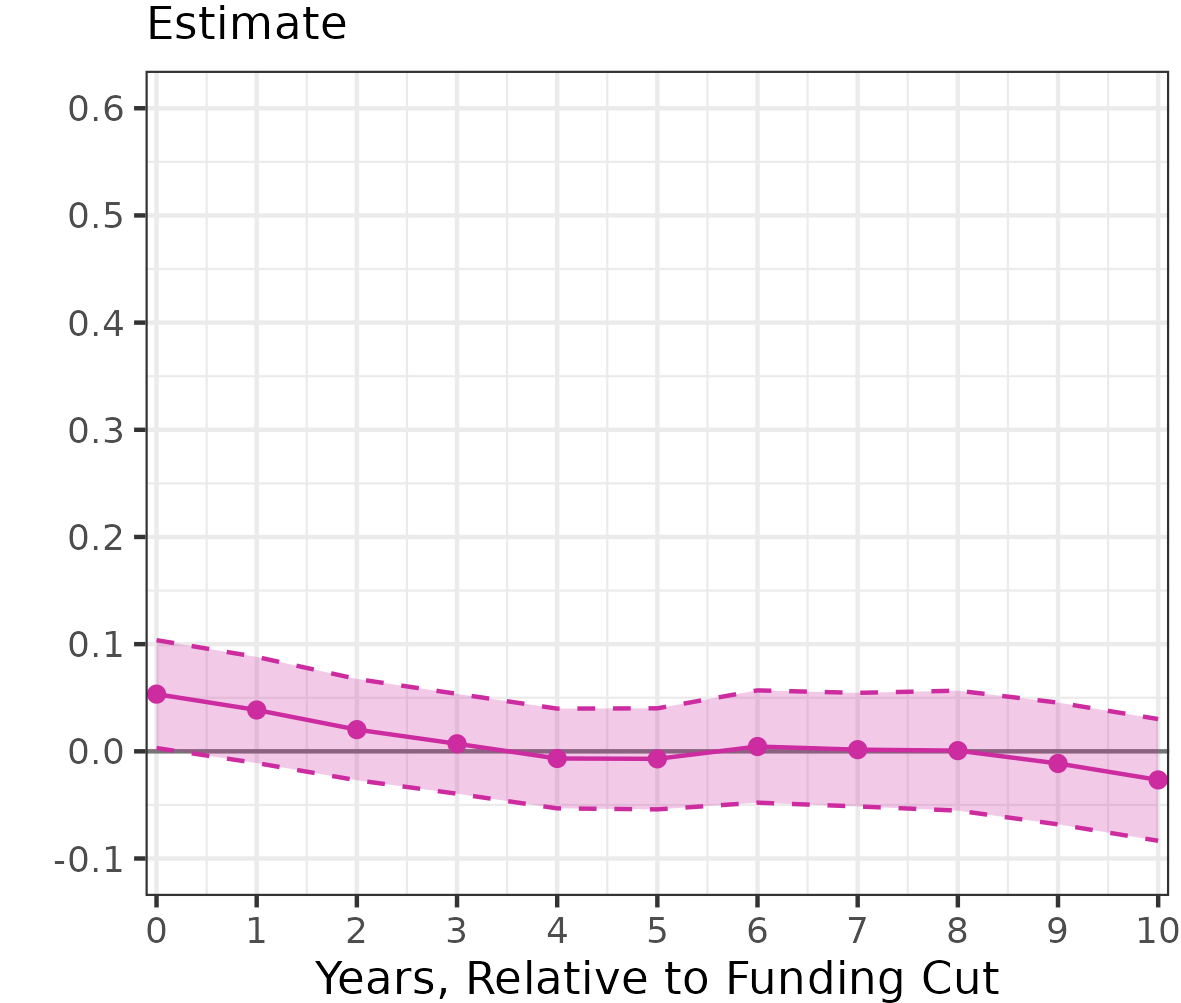
\includegraphics[width=\textwidth]{figures/all-count-lp.png}
        \label{fig:all-count-lp}
    \end{subfigure}
    \label{fig:count-lp}
    \justify
    \footnotesize
    \textbf{Note}:
    These figures show the local projections estimates of regression specification \eqref{eqn:secondstage}, with the funding shock as an instrument for state funding.
    The unit of analysis is the university, and uses IPEDS data.
    The coefficient estimate is effect of state funding ($X_{i,t}$) on faculty count per student ($Y_{i,t}$), using the funding shock instrument ($Z_{i,t}$), while accounting for auto-correlation between different time periods --- i.e., between $X_{i,t}, X_{i,t-1}$ and $Y_{i,t}, Y_{i,t-1}$.
    These results use a $\log-\log$ specification, so the estimates are for the elasticity of professor count per student in a year $t+k$ with respect to state funding in year $t$, where years $k = 0, \hdots, 10$ are on the $x$-axis. 
    Standard errors are clustered at the state-year level.
\end{figure}

\newpage
\begin{figure}[H]
    \centering
    \singlespacing
    \caption{Local Projection Estimates for Effect of State Funding on Faculty Salaries per Student at Illinois Public Universities, by Professor Group.}
    \begin{subfigure}[b]{0.495\textwidth}
        \centering
        \caption{Lecturers.}
        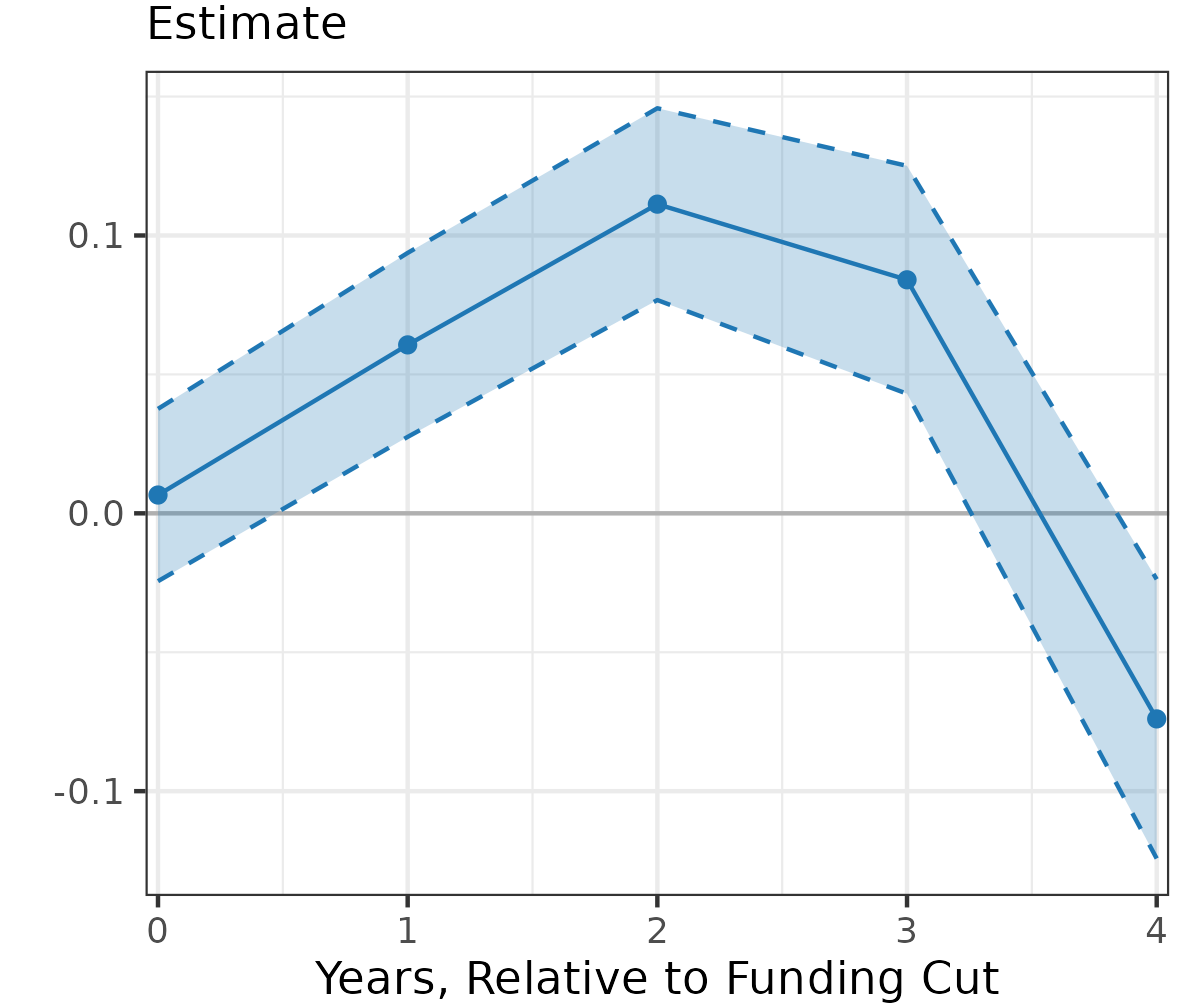
\includegraphics[width=\textwidth]{figures/salaries-lecturer-illinois-lp-rolling.png}
        \label{fig:salaries-lecturer-illinois-lp-rolling}
    \end{subfigure}
    \begin{subfigure}[b]{0.495\textwidth}
        \centering
        \caption{Assistant Professors.}
        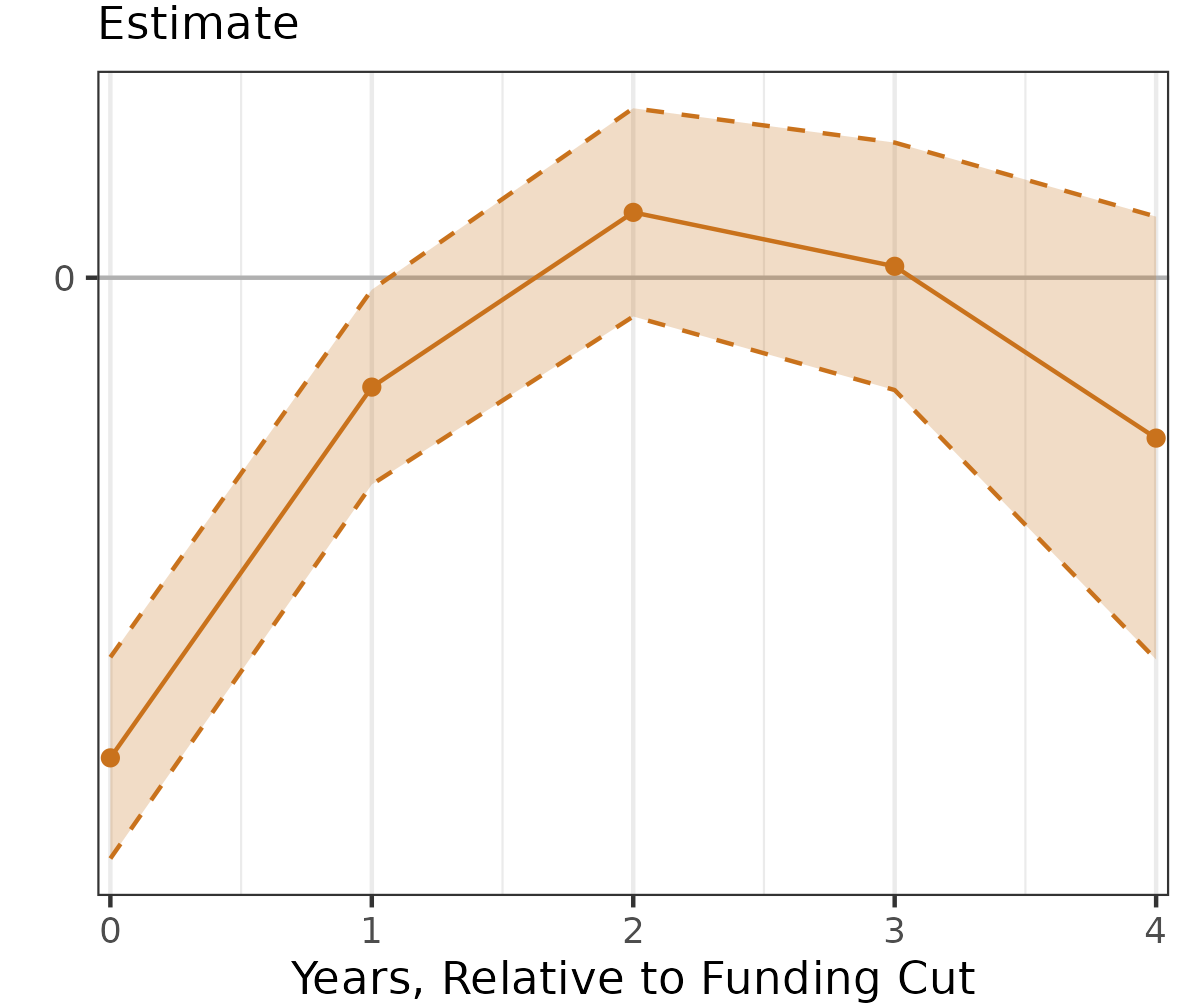
\includegraphics[width=\textwidth]{figures/salaries-assistant-illinois-lp-rolling.png}
        \label{fig:salaries-assistant-illinois-lp-rolling}
    \end{subfigure}
    \begin{subfigure}[b]{0.495\textwidth}
        \centering
        \caption{Full Professors.}
        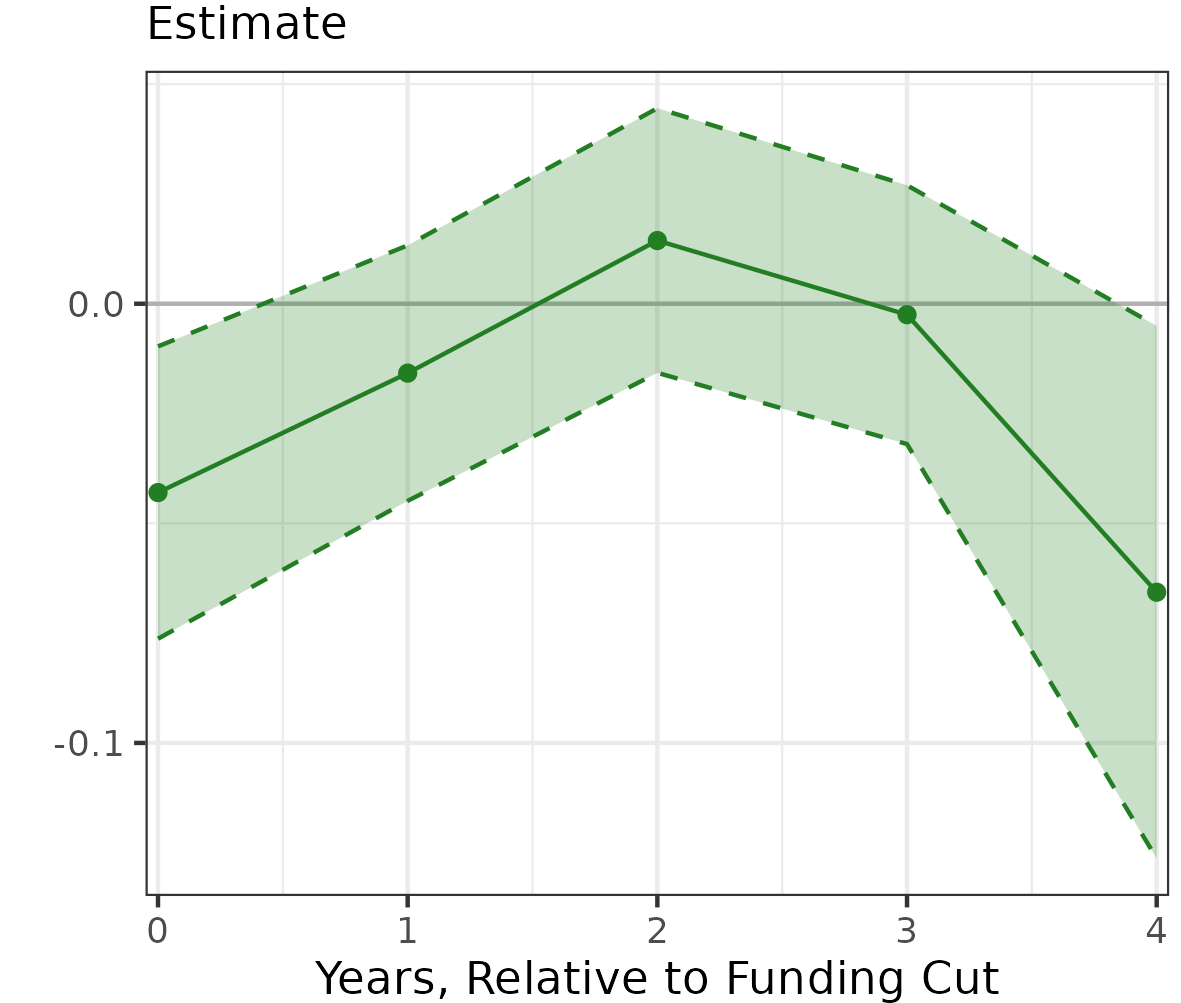
\includegraphics[width=\textwidth]{figures/salaries-full-illinois-lp-rolling.png}
        \label{fig:salaries-full-illinois-lp-rolling}
    \end{subfigure}
    \begin{subfigure}[b]{0.495\textwidth}
        \centering
        \caption{Administrator Professors.}
        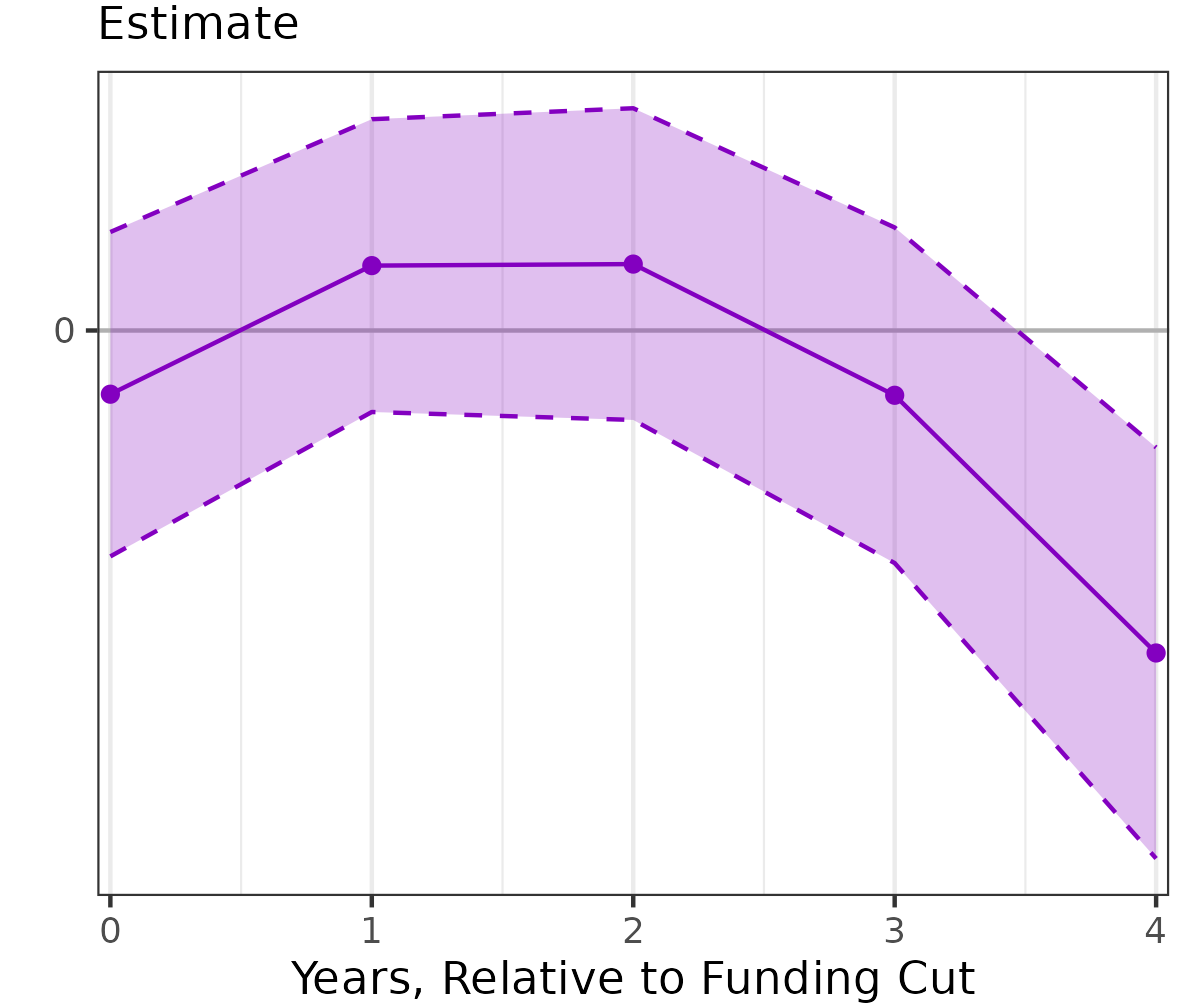
\includegraphics[width=\textwidth]{figures/salaries-administrator-illinois-lp-rolling.png}
        \label{fig:salaries-administrator-illinois-lp-rolling}
    \end{subfigure}
    \label{fig:salaries-illinois-lp-rolling}
    \justify
    \footnotesize
    \textbf{Note}:
    These figures show the local projections estimates of regression specification \eqref{eqn:secondstage}, with the funding shock as an instrument for state funding.
    The unit of analysis is an individual faculty member (at an Illinois public university); funding data come from IPEDS, and faculty salaries from IBHED.
    The coefficient estimate is effect of state funding ($X_{i(j),t}$) on faculty salaries ($Y_{j,t}$), using the funding shock instrument ($Z_{i(j),t}$), while accounting for auto-correlation between different time periods --- i.e., between $X_{i(j),t}, X_{i(j),t-1}$ and $Y_{i(j),t}, Y_{i(j),t-1}$.
    These results use a $\log-\log$ specification, so the estimates are for the elasticity of faculty salaries student in a year $t+k$ with respect to state funding in year $t$, where years $k = 0, \hdots, 4$ are on the $x$-axis. 
    Standard errors are clustered at the university-year level, and \autoref{sec:iv-model-indiv} fully describes the differences in empirical specification when unit of analysis is an individual faculty member.
\end{figure}


%%%%%%%%%%%%%%%%%%%%%%%%%%%%%%%%%%%%%%%%%
%% Section to host Tables
\newpage
\section{Tables}
\label{sec:tables}

\begin{table}[H]
    \singlespacing
    %\centering
    \caption{IPEDS Summary Statistics, Public Universities Panel 1990--2021}
    \makebox[\textwidth][c]{
\begin{tabular}{@{\extracolsep{5pt}}lccc} 
\\[-1.8ex]\hline 
\hline \\[-1.8ex] 
Statistic & \multicolumn{1}{c}{Mean} & \multicolumn{1}{c}{St. Dev.} & \multicolumn{1}{c}{N} \\ 
\hline \\[-1.8ex] 
Enrolment & 11,870 & 10,876 & 17,012 \\ 
State Funding (millions 2021 USD) & 104 & 127 & 17,012 \\ 
Total revenues (millions 2021 USD) & 450 & 818 & 17,012 \\ 
Non-institutional revenues (millions 2021 USD) & 213 & 272 & 17,012 \\ 
Lecturers count & 59 & 73 & 17,012 \\ 
Assistant professors count & 116 & 102 & 17,012 \\ 
Full professors count & 269 & 287 & 17,012 \\ 
All faculty count & 453 & 445 & 17,012 \\ 
\hline \\[-1.8ex] 
\end{tabular} 
}
    \label{tab:ipeds-summary}
    \justify
    \footnotesize
    \textbf{Note}:
    This table shows the summary statistics for every public university--year observation in IPEDS data.
    The numbers are adjusted to 2021 figures by CPI-U.
    Non-institutional revenues refers to the sum of federal, state, and local funding plus tuition revenues; these sum to the majority of university funding, but exclude numbers such as university income from capital projects.
\end{table}

\begin{table}[H]
    \singlespacing
    \centering
    \caption{IBHED Summary Statistics, Professor Panel 2010--2021.}
    \makebox[\textwidth][c]{
\begin{tabular}{@{\extracolsep{5pt}}lccc} 
\\[-1.8ex]\hline 
\hline \\[-1.8ex] 
Statistic & \multicolumn{1}{c}{Mean} & \multicolumn{1}{c}{St. Dev.} & \multicolumn{1}{c}{N} \\ 
\hline \\[-1.8ex] 
Lecturer, percent & 27 & 44 & 187,634 \\ 
Assistant professor, percent & 21 & 41 & 187,634 \\ 
Full professor, percent & 37 & 48 & 187,634 \\ 
Administrator professor, percent & 15 & 36 & 187,634 \\ 
Lecturer salary (2021 USD) & 31,449 & 25,786 & 50,588 \\ 
Assistant salary (2021 USD) & 76,897 & 38,059 & 39,421 \\ 
Full salary (2021 USD) & 109,283 & 48,919 & 68,774 \\ 
Administrator salary (2021 USD) & 119,249 & 61,321 & 28,851 \\ 
All salary (2021 USD) & 83,027 & 55,843 & 187,634 \\ 
Lecturer benefits (2021 USD) & 2,342 & 6,470 & 50,588 \\ 
Assistant benefits (2021 USD) & 2,965 & 7,096 & 39,421 \\ 
Full benefits (2021 USD) & 6,722 & 13,624 & 68,774 \\ 
Administrator benefits (2021 USD) & 3,599 & 15,928 & 28,851 \\ 
All benefits (2021 USD) & 4,272 & 11,513 & 187,634 \\ 
\hline \\[-1.8ex] 
\end{tabular} 
}
    \label{tab:illinois-summary}

    \justify
    \footnotesize
    \textbf{Note}:
    This table shows the summary statistics for every faculty--year observation in the IBHED data, which represents every faculty member in the Illinois public university system over years 2010--2021.
    The numbers are adjusted to 2021 figures by CPI-U.
    Lecturer is a binary for whether the faculty member is designated as a lecturer in the databse, and similarly for the assistant professors, full professors, and administrative faculty;
    salary refers the sum of base salary and benefits.
    All salary and benefits refers to summary statistics on the salary and benefits, respectively, of all faculty (regardless of position).
\end{table}

\newpage
\begin{table}[H]
    \singlespacing
    \centering
    \caption{First Stage Estimates, for State Funding by Funding Shock in IPEDS Data.}
    \textbf{Panel A: units in \$ per student}
    
    \makebox[\textwidth][c]{
\begin{tabular}{@{\extracolsep{5pt}}lcccc} 
\\[-1.8ex]\hline 
\hline \\[-1.8ex] 
 & \multicolumn{4}{c}{Dependent Variable: State Funding} \\ 
\cline{2-5} 
\\[-1.8ex] & (1) & (2) & (3) & (4)\\ 
\hline \\[-1.8ex] 
 Funding Shock & $-$1.176 & $-$0.160 & $-$1.100 & $-$1.071 \\ 
  & (0.226) & (0.265) & (0.242) & (0.264) \\ 
  Tuition Revenue &  &  & $-$0.295 & 1.012 \\ 
  &  &  & (0.136) & (0.329) \\ 
  Constant &  & 9,716.437 &  & $-$1,708.334 \\ 
  &  & (1,805.394) &  & (2,716.150) \\ 
 \hline \\[-1.8ex] 
Uni. + Year fixed effects? & Yes & No & Yes & No \\ 
F stat. & 20.712 & 16.512 & 26.999 & 0.365 \\ 
Observations & 17,012 & 17,012 & 17,012 & 17,012 \\ 
R$^{2}$ & 0.918 & 0.0004 & 0.919 & 0.074 \\ 
\hline 
\hline \\[-1.8ex] 
\end{tabular} 
}
    
    \textbf{Panel B: units in log \$ per student}
    
    \makebox[\textwidth][c]{
\begin{tabular}{@{\extracolsep{5pt}}lcccc} 
\\[-1.8ex]\hline 
\hline \\[-1.8ex] 
 & \multicolumn{4}{c}{Dependent Variable: State Funding} \\ 
\cline{2-5} 
\\[-1.8ex] & (1) & (2) & (3) & (4)\\ 
\hline \\[-1.8ex] 
 Funding Shift-share& $-$0.977 & $-$0.302 & $-$0.986 & $-$0.573 \\ 
  & (0.066) & (0.093) & (0.062) & (0.067) \\ 
  Tuition Revenue &  &  & 0.058 & 0.535 \\ 
  &  &  & (0.059) & (0.065) \\ 
  Constant &  & 6.419 &  & $-$0.484 \\ 
  &  & (0.769) &  & (0.844) \\ 
 \hline \\[-1.8ex] 
Uni. + Year fixed effects? & Yes & No & Yes & No \\ 
F stat. & 249.662 & 74.022 & 218.171 & 10.558 \\ 
Observations & 17,012 & 17,012 & 17,012 & 17,012 \\ 
R$^{2}$ & 0.790 & 0.047 & 0.790 & 0.180 \\ 
\hline 
\hline \\[-1.8ex] 
\end{tabular} 
}

    \label{tab:firststage-reg}
    \justify
    \footnotesize
    \textbf{Note}:
    These tables show the first stage OLS estimates of regression specification \eqref{eqn:firststage}, showing the effect of the funding shock on state funding to gauge performance as an instrument.
    Each observation is a public univeristy-year, in the IPEDS data.
    Panel A shows the effect of an funding shock of \$-1 per student in the state on the number of \$'s of state funding per student at the university --- i.e.,
    \$-1 funding shock per student in the state leads to \$1.176 less state funding per student at the university according to preferred specification column 1.
    Panel B shows the effect of a $-10$\% change funding shock per student in the state on $10$\% change in state funding per student at the university --- i.e.,
    $-10$\% funding shock per student in the state leads to $-9.77$\% less state funding per student at the university according to prefferred specification column 1.        
    Standard errors are clustered at the state-year level, and univeristy $+$ year fixed effects are included where noted.
\end{table}

\newpage
\begin{table}[H]
    \singlespacing
    \centering
    \caption{Effects of Changes in State Funding on University Faculty Composition, IPEDS 1990--2017, OLS and 2SLS Estimates.}

    \textbf{Panel A: units in \$ per student}

    \makebox[\textwidth][c]{
\begin{tabular}{@{\extracolsep{5pt}}lcccccccc} 
\\[-1.8ex]\hline 
\hline \\[-1.8ex] 
 & \multicolumn{8}{c}{Dependent Variable: Faculty Count per 1,000 Students, by Position} \\ 
\cline{2-9} 
\\[-1.8ex] & \multicolumn{2}{c}{Lecturers} & \multicolumn{2}{c}{Asst. Professors} & \multicolumn{2}{c}{Full Professors} & \multicolumn{2}{c}{All Faculty} \\ 
 & OLS & 2SLS & OLS & 2SLS & OLS & 2SLS & OLS & 2SLS \\ 
\\[-1.8ex] & (1) & (2) & (3) & (4) & (5) & (6) & (7) & (8)\\ 
\hline \\[-1.8ex] 
 State Funding & $-$0.451 & $-$5.957 & $-$0.479 & 1.031 & $-$0.104 & 2.288 & $-$1.198 & $-$3.333 \\ 
  & (0.177) & (1.725) & (0.211) & (1.232) & (0.275) & (2.910) & (0.612) & (4.259) \\ 
 \hline \\[-1.8ex] 
Outcome Mean & 59.253 & 59.253 & 116.121 & 116.121 & 269.103 & 269.103 & 452.507 & 452.507 \\ 
Observations & 17,012 & 17,012 & 17,012 & 17,012 & 17,012 & 17,012 & 17,012 & 17,012 \\ 
R$^{2}$ & 0.742 & 0.595 & 0.887 & 0.881 & 0.973 & 0.971 & 0.954 & 0.954 \\ 
\hline 
\hline \\[-1.8ex] 
\end{tabular} 
}
    
    \textbf{Panel B: units in log \$ per student}
    
    \makebox[\textwidth][c]{
\begin{tabular}{@{\extracolsep{5pt}}lcccccccc} 
\\[-1.8ex]\hline 
\hline \\[-1.8ex] 
 & \multicolumn{8}{c}{Dependent Variable: Employment Count by Professor Group} \\ 
\cline{2-9} 
\\[-1.8ex] & \multicolumn{2}{c}{Lecturer} & \multicolumn{2}{c}{Assistant} & \multicolumn{2}{c}{Full} & \multicolumn{2}{c}{All} \\ 
 & OLS & 2SLS & OLS & 2SLS & OLS & 2SLS & OLS & 2SLS \\ 
\\[-1.8ex] & (1) & (2) & (3) & (4) & (5) & (6) & (7) & (8)\\ 
\hline \\[-1.8ex] 
 State Funding & $-$0.137 & $-$0.437 & 0.082 & 0.135 & 0.123 & 0.137 & 0.077 & 0.065 \\ 
  & (0.032) & (0.100) & (0.047) & (0.068) & (0.056) & (0.038) & (0.047) & (0.030) \\ 
 \hline \\[-1.8ex] 
Outcome Mean & 0.572 & 0.572 & 1.194 & 1.194 & 2.298 & 2.298 & 4.128 & 4.128 \\ 
Observations & 17,012 & 17,012 & 17,012 & 17,012 & 17,012 & 17,012 & 17,012 & 17,012 \\ 
R$^{2}$ & 0.660 & 0.646 & 0.705 & 0.704 & 0.797 & 0.797 & 0.810 & 0.810 \\ 
\hline 
\hline \\[-1.8ex] 
\end{tabular} 
}

    \label{tab:facultycount-shock-reg}
    \justify
    \footnotesize
    \textbf{Note}:
    These tables show the second stage OLS and 2SLS estimates of regression specification \eqref{eqn:secondstage}, showing the effect of state funding changes on faculty outcomes, using the funding shock to instrument for state funding in the columns labelled 2SLS.
    Each observation is a public university-year, in the IPEDS data.
    Panel A shows the effect of a fall in state funding \$$-1,000$ per student in the state on the number of professors --- i.e.,
    an extra \$$1,000$ per student leads to 6 fewer lecturers according to column 2.
    Panel B shows the effect of a $10$\% change in state funding per student at the university on the 10\% change in the number of professors per students --- i.e.,
    an extra 10\% of state funding per student leads to 4.37\% fewer lecturers per student according to column 2.
    Outcome-mean is the mean of the outcome, for Panel A the number of professors per student, for Panel B the number of faculty per student.
    Panel B uses $\log$ faculty count per student as the outcome, though the outcome mean is count of faculty per student (not in $\log$ terms).
    Standard errors are clustered at the state-year level, and university $+$ year fixed effects are included through--out.
\end{table}

\newpage
\begin{table}[H]
    \singlespacing
    \centering
    \caption{Effects of Changes in State Funding on Faculty Salaries and Exit Rate, in Illinois 2010--2021, 2SLS Estimates.}
    \label{tab:faculty-shock-illinois-rolling}
    \makebox[\textwidth][c]{
\begin{tabular}{@{\extracolsep{5pt}}lccccc} 
\\[-1.8ex]\hline 
\hline \\[-1.8ex] 
 & \multicolumn{5}{c}{Dependent Variable: Annual Salaries} \\ 
\cline{2-6} 
 & Lecturer & Assistant & Full & Admin & All \\ 
\\[-1.8ex] & (1) & (2) & (3) & (4) & (5)\\ 
\hline \\[-1.8ex] 
 State Funding & 0.007 & $-$0.072 & $-$0.043 & $-$0.010 & $-$0.012 \\ 
  & (0.095) & (0.041) & (0.038) & (0.049) & (0.086) \\ 
 \hline \\[-1.8ex] 
Observations & 26,324 & 22,328 & 9,065 & 11,529 & 69,246 \\ 
R$^{2}$ & 0.220 & 0.051 & 0.069 & 0.144 & 0.163 \\ 
\hline 
\hline \\[-1.8ex] 
\end{tabular} 
}
    
    \makebox[\textwidth][c]{
\begin{tabular}{@{\extracolsep{5pt}}lccccc} 
\\[-1.8ex]\hline 
\hline \\[-1.8ex] 
 & \multicolumn{5}{c}{Dependent Variable: Exit rate by Professor Group} \\ 
\cline{2-6} 
 & Lecturer & Assistant & Full & Admin & All \\ 
\\[-1.8ex] & (1) & (2) & (3) & (4) & (5)\\ 
\hline \\[-1.8ex] 
 State Funding & $-$0.003 & 0.003 & $-$0.002 & $-$0.003 & $-$0.004 \\ 
  & (0.024) & (0.007) & (0.009) & (0.020) & (0.016) \\ 
 \hline \\[-1.8ex] 
Observations & 23,841 & 19,904 & 7,244 & 10,241 & 61,230 \\ 
R$^{2}$ & 0.013 & 0.005 & 0.013 & 0.072 & 0.016 \\ 
\hline 
\hline \\[-1.8ex] 
\end{tabular} 
}

    \makebox[\textwidth][c]{
\begin{tabular}{@{\extracolsep{5pt}}lcccc} 
\\[-1.8ex]\hline 
\hline \\[-1.8ex] 
 & \multicolumn{4}{c}{Dependent Variable: Promotion Rate by Professor Group} \\ 
\cline{2-5} 
 & Lecturer & Assistant & Associate & All \\ 
\\[-1.8ex] & (1) & (2) & (3) & (4)\\ 
\hline \\[-1.8ex] 
 State Funding & 0.015 & 0.036 & 0.029 & 0.016 \\ 
  & (0.007) & (0.019) & (0.065) & (0.008) \\ 
 \hline \\[-1.8ex] 
Observations & 16,420 & 16,972 & 4,340 & 42,132 \\ 
R$^{2}$ & 0.008 & 0.022 & 0.031 & 0.007 \\ 
\hline 
\hline \\[-1.8ex] 
\end{tabular} 
}

    \justify
    \footnotesize
    \textbf{Note}: 
    These tables show the second stage 2SLS estimates of regression specification \eqref{eqn:secondstage}, showing the effect of state funding changes on faculty outcomes at Illinois universities, using the funding shock to instrument for state funding.
    The shift-share instrument is based in the year the professor was hired, following definition in \autoref{sec:iv-model-indiv}.
    Each observation is a faculty member--year at an Illinois public university, where funding data come from IPEDS and faculty outcomes from IBHED data.
    The panels shows the effect of a $1$\% change in state funding per student at the university on faculties' salaries (base salary $+$ benefits), promotion rate (e.g., assistant professor to associate professor), and rate of leaving their university (i.e., by quitting, retiring, or moving to another university).
    Standard errors are clustered at the university-year of hire level, and university $+$ year of hire fixed effects are included through--out.
\end{table}
